\chapter{Simulations}
In this chapter, we detail simulations that we developed to test our hypothesis with a complete implementation of K-HAS. LORIS was implemented because current technology does not fully support the requirements of the K-HAS architecture, because of this we implemented a simulation of K-HAS that satisfies all of its requirements.

Using RePast, a java-based network simulation tool, we created a network to emulate K-HAS. Repast is an agent-based modelling system that allows for agents to be created and placed on a grid. Ticks denote a period of time and simulations can run for a fixed number of ticks, or until stopped. Ticks can also be used to schedule events, such as searching for neighbours, by calling methods that last for a set number of ticks, or begin at a particular tick. Similar to the chaining of rules we described with Drools, ticks are the core of Repast's scheduling mechanism which can be used to schedule single events, as well as chaining events. Consider a train simulation. A train may take three hundred ticks to arrive at its destination, from the train arrival a scheduled event to open doors and make announcements which could schedule other events and so on.

Agents are created, using the RePast SDK and Java classes are used to manipulate their behaviour. Simple networks may only contain basic agents with only a few variations from those provided by RePast. However, for more complex networks, a hierarchy of agents is required and Java's inheritance can then be used create subclasses of an agent.

A 2D (or 3D) space is used to display the grid and the simulation is run within Repast's own GUI, that provides functionality such as editing the properties of classes, integrating with Matlab, taking screenshots and saving different configurations of the same network.

The rest of this chapter is structured as follows. Section 2 describes the implementation of the network. Section 3 outlines the results and Section 4 compares these with LORIS and the current solution in our motivating scenario. Section 5 concludes our findings and highlights areas that require further experimentation.

\section{K-HAS Implementation}
As described in Chapter \ref{chap:arch}, K-HAS consists of three tiers: Data Collection, Data Processing and Data Aggregation. The DC tier focusses on capturing sensed data, performing basic processing and routing sensed data to the DP tier. The DP tier has more knowledge-processing capabilities and nodes are responsible for processing sensed data. Using a rule engine and a dynamic knowledge base, DP nodes process more than just the metadata of sensed data in order to create a classification. DP nodes have a direct connection to the DA node, which is the the endpoint in the K-HAS network, an Internet connected node that stores all sensed data from the network and acts as the central knowledge base.

K-HAS was originally intended to be deployed around Danau Girang and, over the course of three years, we have collected several thousand images and local knowledge interviews in order to configure K-HAS before deployment. Because of this, the data we have collected was used to create a deployment of K-HAS using scientific observations, in order to fit with our motivating scenario. LORIS had already been deployed to capture scientific observations, so this made a comparison of the three (current manual solution, LORIS and K-HAS simulation) possible and because we already had metrics on areas of the network such as battery life, transmission time of a Darwin Core archive and processing time.

Before implementing, we designed the agents required based largely on the existing ontology. Using that, we created a hierarchy of nodes inheriting common properties from a node object. As previously mentioned, we had metrics on range and transmission times from previous experiments and the deployment of LORIS, we used these to create properties for each transmission medium that could be used by each node object.

We also needed to create an object to represent the DwC archives, a Drools REST API had been implemented to work with the LORIS web interface, and much of the DwC archive code was reusable within RePast. 

The structure of the simulation is shown below. Network builder instantiates all the nodes, places them on randomly on the grid and schedules events once the simulation has started. The nodes then use the properties of their transmission medium to find nodes in range and create a connection, depicted by a line between the node. The simulation can be run in one of two modes: random or based on a 2010 DG deployment. 

DG mode means that it models a 6 month deployment in Danau Girang from 2010. All images taken in that time had the time they were taken, the original camera ID and the size of each image recorded into a CSV file. This file is read by the Network Builder and the contents are provided to each node. The first tick starts at the same time as the first image is taken. The number of deployed nodes matches the number of deployed cameras and, upon each tick, they check whether an image was taken by them at that tick. If so, an image is captured, archived and forwarded to the nearest DP node. This process runs, using the scheduler in RePast, for the six month deployment and the details of each archive (time captured, size, route taken, time taken to reach DA node) is saved into a CSV file when it reaches the DA node. Once the six month deployment has run, the simulation can either stop or continue randomly.

The random mode uses metrics extracted from the images taken at Danau Girang, but the chance of an image being captured at a camera is based on the average capture rate of a camera. The fire rate has been calculated by the average number of pictures captured in a day taken by each camera. 

\begin{itemize}
\item Network Builder
\item Node
	\begin{itemize}
	\item Data Collection
	\item Data Processing
	\item Data Aggregation
	\end{itemize}
\item Darwin Core
	\begin{itemize}
	\item Identification
	\item Location
	\item Occurrence
	\item Image
	\item Species
	\end{itemize}	 
\end{itemize}

\subsection{Darwin Core}
The Darwin Core class represents a DwC archive, encapsulation Identification, Location, Occurrence, Image and Species. The images we have collected from Danau Girang were processed to find details such as the average size when taking at night and day, how often an average camera triggers and the percentage of images with animal content. These data were then used to specify how often a randomly placed node should capture an observation per tick.

Upon each capture, and based on the `time' of day, images are created, given a random size based on the maximum and minimum size found in the 120,000 images collected from DG and the sum of the images is used to calculate the size of the archive. Using this size, a DC node calculates how long the archive takes to send based on the size and the transmission rate, we assume that the rate stays constant for the duration of transmission.
When an archive is sent to the DP node, we used the average time for our image processing tool and Drools engine to run and attempt a classification, which is 143 seconds (ticks). To keep the classifications as general as possible, so that the simulation applies to any WSN for scientific observations, archives are not classified down to the species level, they are marked as \textit{interesting} or \textit{empty} and then forwarded to the DA node.

\subsection{Routing}
The routing protocol used by K-HAS needs to be dynamic in order to adapt to nodes being added and removed during deployment, while minimising traffic in a resource constrained network. The approach we use a modification the Minimum Cost Forwarding Algorithm (MCFA), described in Section \ref{bg:rp}. A cost is assigned to each node, based on how far they are from the DA node, with neighbouring nodes choosing to connect to the node with the lowest cost. However, in normal implementations of MCFA, all nodes are of the same type and simply need to connect to a base station.

In K-HAS, DC nodes cannot connect directly to a DA node, because processing would not take place. K-HAS MCFA works with a discovery phase and a transmission phase. The discovery phase is a scheduled event, taking place at the start of deployment but it can be run throughout deployment to react to nodes being added or removed. 

\subsubsection{Discovery}
	Discovery begins at each DA node, scanning nodes in range for DP nodes and sending a broadcast packet with a cost of 0 to inform them that they are within range of a DA node which, in our implementation, uses Wi-Fi. Once received, DP nodes increment the count and forward the packet to any DC nodes within range of them, where we use the range of Digimesh. We found that this method overloaded the DP nodes and all DC nodes within range would connect to the first DP node they receive the broadcast from. We then implemented a method, called \textit{load balancing}, which uses the DC nodes connected to a DP node to calculate whether it should offload new nodes to a neighbouring DP node.
	
	The maximum connections a DP node can have is determined by the total number of DC nodes in the network divided by the total number of DP nodes, which is held in the knowledge base of the DA node. Once a DP node has the maximum number of connections allowed, it starts to offload to a neighbouring DP node that is also in range of the DC node requesting a connection. If there are no neighbouring nodes then it simply goes over the maximum number of connections allowed, to save DC nodes being left with nowhere to send their data.
	
	If the DC node that receives the broadcast does not have an existing route to a DA node, or the cost of the current route is higher than the received route, it adds an edge to the DP node, increments the count and forwards it to all nodes in range. This process continues until the broadcast reaches the edge of the network. Nodes do not have global knowledge of the route to the DA node, only of their neighbour with the lowest cost.
	
	This phase can be repeated throughout the course of the deployment, simply by scheduling it as an event to occur every \textit{n} ticks. However, the simulation currently only uses the discovery phase at the beginning of the deployment.
	
\subsubsection{Transmission}
	Once the discovery phase has been completed, providing nodes are within range of the DA node, the transmission phase begins where only DwC archives are then sent across the network. Observations are captured based on the mode of the simulation and sent to the lowest cost neighbour.
	
	In order to manage transmissions, DC nodes have a \textit{SendState} object that contains the next archive to send, the time to send it and whether it is currently sending. This is used to determine what operations to perform, once an archive has been sent, it is delete from the SendState and the sending flag is set to false. A new archive is then added and sent when the opportunity arises.
	
	When a DP node receives the archive, it begins processing and we have implemented both sending and processing as serial processes. DP nodes use the SendState as well, but they do not add any archive, they add an archive once it has been processed and they then select the oldest archive that has been classified as interesting, providing that an archive is not already waiting to be sent. The archive stores information about the route it takes, recording every hop, as well as the time it took from capture to DA node.
	
	Scheduled sending events run every thousand ticks, which is configurable, to check the sending state of the node and send any archives in the SendState. The node then waits for the number of ticks that it will take in order to transmit the archive.
	
	Once the simulation is completed, either manually or through a defined number of ticks, the archives in each DA node are iterated over and written to a CSV file, with details like the path it took, total transmission time and time of capture.
	
\subsection{Capture}
	Using the existing data collected from Danau Girang, we calculated how often a camera triggers in a six month deployment, as well as how often the observation contained interesting content. 
	
	To calculate the count of interesting images, we processed every directory of images to extract the largest object in the foreground, using our Triton program. Once processed, we iterated through every directory, counted the total number of images and the total number of extracted images. We then calculated the average for each directory and then summed those averages divided by the total number of directories. This gave us a 20.7\% chance of an image being interesting.
	
	The chance of camera trigger was calculated by the total number of observations (13,399) divided by the number of seconds in six months (15,552,000). This gives a chance of 0.000861561. A random number is generated every and compared to this, if the value is fewer than or equal to the chance, then an observation is captured.

\section{Results}
	As previously explained, the simulation runs in a random mode, or using data from an existing deployment. We added a property that ensured each simulation only ran for 15,552,000 seconds, simulating a six month deployment.
	
	Before any experiments were run, we calculated the transmission time for the current solution at Danau Girang. Using the creation date of each image, and the date that the SD card was collected, we found the average number of hours between capture and being received at the field centre, which was 491 hours. It should be noted that this time does not include the upload or processing of each archive, but there was no accurate way of calculating this, and it does not distinguish between empty and interesting observations.
	
	 We performed one hundred runs in which the simulation recorded between 57,000 and 60,000 observations in each run. At the end of each run, a CSV file is written with the details of each observation that is stored on every DA node; it does not take undelivered observations into account. After counting the observations, we calculate the total interesting images and their average time to be delivered. The runs resulted in an average transmission time of 49.3 hours for interesting observations and 2043 hours for empty observations. Figure \ref{fig:sim} shows the view of the simulation, with a list of the properties that can be set.
	
	\begin{figure}[h]
	\centering
	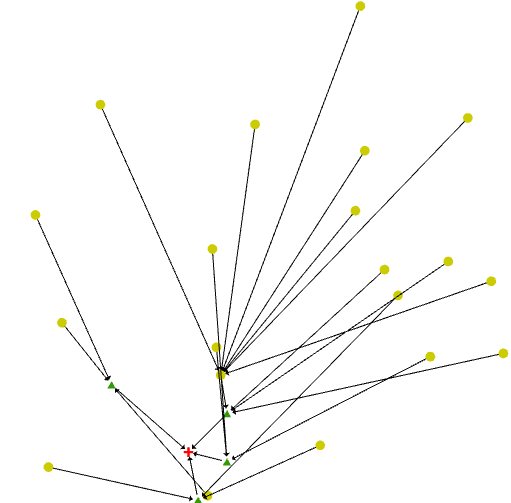
\includegraphics[width=0.70\textwidth]{Chap7/figures/khas_sim}
	\caption{K-HAS Simulation}
	\label{fig:sim}
	\end{figure}
	
	**COMPARE TO LORIS HERE?**

	
\section{Improvements}
Although the simulations do show an improvement over the current implementation, there are features that could be added to ensure that the simulation models a real-world implementation as closely as possible. Currently, the processing time of DP nodes is based on the average time to process an archive, using a random time within a range would make this less static. 

All nodes within the network do not use a battery life and, due to the short deployment time of LORIS, we do not have accurate information on how long batteries last on each node. This is most important on DC nodes as there may be hundreds deployed at any one time and the DA node must report when a DC node does not report for a while. This also goes for transmission, using a fixed range and transfer rate suits a dynamic network in an open environment but obstacles and weather affect the rate and this could be taken into account in a future implementation.

In our implementation of K-HAS, we are using image-based scientific observations but the chance of a camera being triggered is the same for every DC node. In a future version, it would be more realistic to use different chances of triggering based on the cameras location, or based on random assignments. However, we believe that a more general, extensible simulation that was able to handle many different types of sensed data would be the truest model of K-HAS; using property files, as we currently do, to provide details on the sensed data, processing times and a knowledge base.

\section{Conclusion}
In this chapter we have detailed the development and results of our simulation of the K-HAS architecture. Current technology limits the implementation of the original architecture we developed, so using a simulation framework is the best alternative. We have modelled all variables based on existing data from our motivating scenario and results have shown that using knowledge bases on deployed nodes for the processing of observations within the network allows `interesting' sensed data to be prioritised and delivered to a DA node more than four hundred hours earlier than a manual solution; which does not include human processing time.

While the simulation is not feature complete, we believe it is accurate enough to show how K-HAS utilises the knowledge-processing capabilities at each tier to process, and prioritise, sensed data based on knowledge gained from the environment, previously sensed data and from humans using the network.

